\documentclass[]{article}
\usepackage{lmodern}
\usepackage{amssymb,amsmath}
\usepackage{ifxetex,ifluatex}
\usepackage{fixltx2e} % provides \textsubscript
\ifnum 0\ifxetex 1\fi\ifluatex 1\fi=0 % if pdftex
  \usepackage[T1]{fontenc}
  \usepackage[utf8]{inputenc}
\else % if luatex or xelatex
  \ifxetex
    \usepackage{mathspec}
  \else
    \usepackage{fontspec}
  \fi
  \defaultfontfeatures{Ligatures=TeX,Scale=MatchLowercase}
\fi
% use upquote if available, for straight quotes in verbatim environments
\IfFileExists{upquote.sty}{\usepackage{upquote}}{}
% use microtype if available
\IfFileExists{microtype.sty}{%
\usepackage{microtype}
\UseMicrotypeSet[protrusion]{basicmath} % disable protrusion for tt fonts
}{}
\usepackage[margin=1in]{geometry}
\usepackage{hyperref}
\hypersetup{unicode=true,
            pdftitle={The Effect of Vitamin C on Tooth Growth in Guinea Pigs - interpretation of R dataset ToothGrowth},
            pdfauthor={Nikolaos Perdikis},
            pdfborder={0 0 0},
            breaklinks=true}
\urlstyle{same}  % don't use monospace font for urls
\usepackage{color}
\usepackage{fancyvrb}
\newcommand{\VerbBar}{|}
\newcommand{\VERB}{\Verb[commandchars=\\\{\}]}
\DefineVerbatimEnvironment{Highlighting}{Verbatim}{commandchars=\\\{\}}
% Add ',fontsize=\small' for more characters per line
\usepackage{framed}
\definecolor{shadecolor}{RGB}{248,248,248}
\newenvironment{Shaded}{\begin{snugshade}}{\end{snugshade}}
\newcommand{\AlertTok}[1]{\textcolor[rgb]{0.94,0.16,0.16}{#1}}
\newcommand{\AnnotationTok}[1]{\textcolor[rgb]{0.56,0.35,0.01}{\textbf{\textit{#1}}}}
\newcommand{\AttributeTok}[1]{\textcolor[rgb]{0.77,0.63,0.00}{#1}}
\newcommand{\BaseNTok}[1]{\textcolor[rgb]{0.00,0.00,0.81}{#1}}
\newcommand{\BuiltInTok}[1]{#1}
\newcommand{\CharTok}[1]{\textcolor[rgb]{0.31,0.60,0.02}{#1}}
\newcommand{\CommentTok}[1]{\textcolor[rgb]{0.56,0.35,0.01}{\textit{#1}}}
\newcommand{\CommentVarTok}[1]{\textcolor[rgb]{0.56,0.35,0.01}{\textbf{\textit{#1}}}}
\newcommand{\ConstantTok}[1]{\textcolor[rgb]{0.00,0.00,0.00}{#1}}
\newcommand{\ControlFlowTok}[1]{\textcolor[rgb]{0.13,0.29,0.53}{\textbf{#1}}}
\newcommand{\DataTypeTok}[1]{\textcolor[rgb]{0.13,0.29,0.53}{#1}}
\newcommand{\DecValTok}[1]{\textcolor[rgb]{0.00,0.00,0.81}{#1}}
\newcommand{\DocumentationTok}[1]{\textcolor[rgb]{0.56,0.35,0.01}{\textbf{\textit{#1}}}}
\newcommand{\ErrorTok}[1]{\textcolor[rgb]{0.64,0.00,0.00}{\textbf{#1}}}
\newcommand{\ExtensionTok}[1]{#1}
\newcommand{\FloatTok}[1]{\textcolor[rgb]{0.00,0.00,0.81}{#1}}
\newcommand{\FunctionTok}[1]{\textcolor[rgb]{0.00,0.00,0.00}{#1}}
\newcommand{\ImportTok}[1]{#1}
\newcommand{\InformationTok}[1]{\textcolor[rgb]{0.56,0.35,0.01}{\textbf{\textit{#1}}}}
\newcommand{\KeywordTok}[1]{\textcolor[rgb]{0.13,0.29,0.53}{\textbf{#1}}}
\newcommand{\NormalTok}[1]{#1}
\newcommand{\OperatorTok}[1]{\textcolor[rgb]{0.81,0.36,0.00}{\textbf{#1}}}
\newcommand{\OtherTok}[1]{\textcolor[rgb]{0.56,0.35,0.01}{#1}}
\newcommand{\PreprocessorTok}[1]{\textcolor[rgb]{0.56,0.35,0.01}{\textit{#1}}}
\newcommand{\RegionMarkerTok}[1]{#1}
\newcommand{\SpecialCharTok}[1]{\textcolor[rgb]{0.00,0.00,0.00}{#1}}
\newcommand{\SpecialStringTok}[1]{\textcolor[rgb]{0.31,0.60,0.02}{#1}}
\newcommand{\StringTok}[1]{\textcolor[rgb]{0.31,0.60,0.02}{#1}}
\newcommand{\VariableTok}[1]{\textcolor[rgb]{0.00,0.00,0.00}{#1}}
\newcommand{\VerbatimStringTok}[1]{\textcolor[rgb]{0.31,0.60,0.02}{#1}}
\newcommand{\WarningTok}[1]{\textcolor[rgb]{0.56,0.35,0.01}{\textbf{\textit{#1}}}}
\usepackage{graphicx,grffile}
\makeatletter
\def\maxwidth{\ifdim\Gin@nat@width>\linewidth\linewidth\else\Gin@nat@width\fi}
\def\maxheight{\ifdim\Gin@nat@height>\textheight\textheight\else\Gin@nat@height\fi}
\makeatother
% Scale images if necessary, so that they will not overflow the page
% margins by default, and it is still possible to overwrite the defaults
% using explicit options in \includegraphics[width, height, ...]{}
\setkeys{Gin}{width=\maxwidth,height=\maxheight,keepaspectratio}
\IfFileExists{parskip.sty}{%
\usepackage{parskip}
}{% else
\setlength{\parindent}{0pt}
\setlength{\parskip}{6pt plus 2pt minus 1pt}
}
\setlength{\emergencystretch}{3em}  % prevent overfull lines
\providecommand{\tightlist}{%
  \setlength{\itemsep}{0pt}\setlength{\parskip}{0pt}}
\setcounter{secnumdepth}{0}
% Redefines (sub)paragraphs to behave more like sections
\ifx\paragraph\undefined\else
\let\oldparagraph\paragraph
\renewcommand{\paragraph}[1]{\oldparagraph{#1}\mbox{}}
\fi
\ifx\subparagraph\undefined\else
\let\oldsubparagraph\subparagraph
\renewcommand{\subparagraph}[1]{\oldsubparagraph{#1}\mbox{}}
\fi

%%% Use protect on footnotes to avoid problems with footnotes in titles
\let\rmarkdownfootnote\footnote%
\def\footnote{\protect\rmarkdownfootnote}

%%% Change title format to be more compact
\usepackage{titling}

% Create subtitle command for use in maketitle
\providecommand{\subtitle}[1]{
  \posttitle{
    \begin{center}\large#1\end{center}
    }
}

\setlength{\droptitle}{-2em}

  \title{The Effect of Vitamin C on Tooth Growth in Guinea Pigs - interpretation
of R dataset ToothGrowth}
    \pretitle{\vspace{\droptitle}\centering\huge}
  \posttitle{\par}
    \author{Nikolaos Perdikis}
    \preauthor{\centering\large\emph}
  \postauthor{\par}
      \predate{\centering\large\emph}
  \postdate{\par}
    \date{18 7 2019}


\begin{document}
\maketitle

\hypertarget{summary}{%
\subsection{Summary}\label{summary}}

The response is the length of odontoblasts (cells responsible for tooth
growth) in 60 guinea pigs. Each animal received one of three dose levels
of vitamin C (0.5, 1, and 2 mg/day) by one of two delivery methods,
orange juice or ascorbic acid (a form of vitamin C and coded as VC).

Usage

ToothGrowth

Format

A data frame with 60 observations on 3 variables.\\
{[},1{]} len numeric Tooth length\\
{[},2{]} supp factor Supplement type (VC or OJ).\\
{[},3{]} dose numeric Dose in milligrams/day

\hypertarget{load-the-toothgrowth-data-and-perform-some-basic-exploratory-data-analyses}{%
\subsection{Load the ToothGrowth data and perform some basic exploratory
data
analyses}\label{load-the-toothgrowth-data-and-perform-some-basic-exploratory-data-analyses}}

\begin{Shaded}
\begin{Highlighting}[]
\KeywordTok{library}\NormalTok{(datasets)}
\KeywordTok{library}\NormalTok{(ggplot2)}
\KeywordTok{library}\NormalTok{(dplyr)}
\end{Highlighting}
\end{Shaded}

\begin{verbatim}
## 
## Attaching package: 'dplyr'
\end{verbatim}

\begin{verbatim}
## The following objects are masked from 'package:stats':
## 
##     filter, lag
\end{verbatim}

\begin{verbatim}
## The following objects are masked from 'package:base':
## 
##     intersect, setdiff, setequal, union
\end{verbatim}

\begin{Shaded}
\begin{Highlighting}[]
\KeywordTok{data}\NormalTok{(ToothGrowth)}
\NormalTok{df_TD <-}\StringTok{ }\NormalTok{ToothGrowth}
\CommentTok{#Display the summary of the dataframe}
\KeywordTok{summary}\NormalTok{(df_TD)}
\end{Highlighting}
\end{Shaded}

\begin{verbatim}
##       len        supp         dose      
##  Min.   : 4.20   OJ:30   Min.   :0.500  
##  1st Qu.:13.07   VC:30   1st Qu.:0.500  
##  Median :19.25           Median :1.000  
##  Mean   :18.81           Mean   :1.167  
##  3rd Qu.:25.27           3rd Qu.:2.000  
##  Max.   :33.90           Max.   :2.000
\end{verbatim}

\begin{Shaded}
\begin{Highlighting}[]
\CommentTok{#Display the unique values of dose}
\KeywordTok{unique}\NormalTok{(df_TD}\OperatorTok{$}\NormalTok{dose)}
\end{Highlighting}
\end{Shaded}

\begin{verbatim}
## [1] 0.5 1.0 2.0
\end{verbatim}

\hypertarget{provide-a-basic-summary-of-the-data}{%
\subsection{Provide a basic summary of the
data}\label{provide-a-basic-summary-of-the-data}}

\begin{Shaded}
\begin{Highlighting}[]
\NormalTok{df_TD}\OperatorTok{$}\NormalTok{dose <-}\StringTok{ }\KeywordTok{as.factor}\NormalTok{(df_TD}\OperatorTok{$}\NormalTok{dose)}
\KeywordTok{table}\NormalTok{(df_TD}\OperatorTok{$}\NormalTok{supp,df_TD}\OperatorTok{$}\NormalTok{dose)}
\end{Highlighting}
\end{Shaded}

\begin{verbatim}
##     
##      0.5  1  2
##   OJ  10 10 10
##   VC  10 10 10
\end{verbatim}

\hypertarget{basic-stats-so-mean}{%
\subsection{Basic stats, so mean:}\label{basic-stats-so-mean}}

\begin{Shaded}
\begin{Highlighting}[]
\KeywordTok{mean}\NormalTok{(df_TD}\OperatorTok{$}\NormalTok{len)}
\end{Highlighting}
\end{Shaded}

\begin{verbatim}
## [1] 18.81333
\end{verbatim}

and standard deviation:

\begin{Shaded}
\begin{Highlighting}[]
\KeywordTok{sd}\NormalTok{(df_TD}\OperatorTok{$}\NormalTok{len)}
\end{Highlighting}
\end{Shaded}

\begin{verbatim}
## [1] 7.649315
\end{verbatim}

What does the table above tell us? We confirm the description of the
dataset, as our dataframe contains a total of 60 observations, of 3
different dosage levels and two different supplement types. Let's see
how this all looks in a graph:

\begin{Shaded}
\begin{Highlighting}[]
\NormalTok{plot <-}\StringTok{ }\KeywordTok{ggplot}\NormalTok{(df_TD, }
               \KeywordTok{aes}\NormalTok{(}\DataTypeTok{x=}\NormalTok{dose,}\DataTypeTok{y=}\NormalTok{len,}\DataTypeTok{fill=}\NormalTok{dose))}
\NormalTok{plot }\OperatorTok{+}\StringTok{ }\KeywordTok{geom_boxplot}\NormalTok{(}\DataTypeTok{notch=}\OtherTok{FALSE}\NormalTok{) }\OperatorTok{+}\StringTok{ }\KeywordTok{facet_grid}\NormalTok{(.}\OperatorTok{~}\NormalTok{supp) }\OperatorTok{+}
\StringTok{     }\KeywordTok{scale_x_discrete}\NormalTok{(}\StringTok{"Dosage [mg/day]"}\NormalTok{) }\OperatorTok{+}\StringTok{   }
\StringTok{     }\KeywordTok{scale_y_continuous}\NormalTok{(}\StringTok{"Teeth Growth"}\NormalTok{) }\OperatorTok{+}\StringTok{  }
\StringTok{     }\KeywordTok{ggtitle}\NormalTok{(}\StringTok{"Effect of Dosage and Supplement Type"}\NormalTok{) }\OperatorTok{+}
\StringTok{     }\KeywordTok{scale_fill_brewer}\NormalTok{(}\DataTypeTok{palette=}\StringTok{"Blues"}\NormalTok{)}
\end{Highlighting}
\end{Shaded}

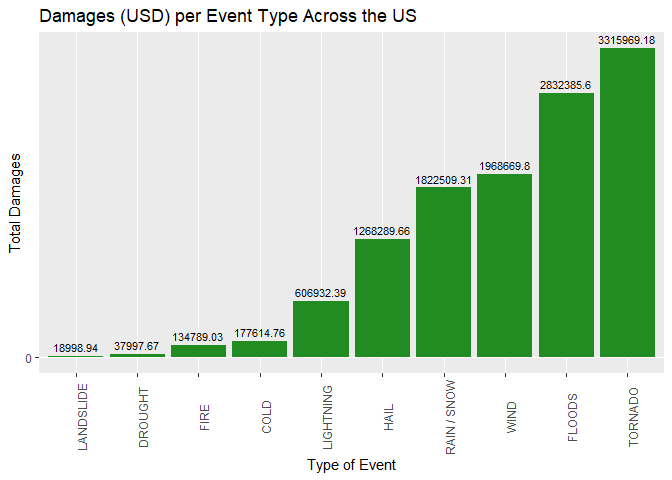
\includegraphics{StatInfCP2_files/figure-latex/unnamed-chunk-4-1.pdf}
While some elements and relationships are clearly visible in the
graphic, let's create some filters and summaries:\\
Get the mean length of toothgrowth, as a function of dose quantity and
type of supplementation:

\begin{Shaded}
\begin{Highlighting}[]
\NormalTok{TG_}\DecValTok{1}\NormalTok{ <-}\StringTok{ }\NormalTok{df_TD }\OperatorTok\StringTok{ }
\StringTok{    }\KeywordTok{group_by}\NormalTok{(supp,dose) }\OperatorTok
\StringTok{    }\KeywordTok{summarize}\NormalTok{(}\DataTypeTok{mean=}\KeywordTok{mean}\NormalTok{(len), }\DataTypeTok{stdev=}\KeywordTok{sd}\NormalTok{(len), }\DataTypeTok{count =} \KeywordTok{n}\NormalTok{())}
\KeywordTok{print}\NormalTok{(TG_}\DecValTok{1}\NormalTok{)}
\end{Highlighting}
\end{Shaded}

\begin{verbatim}
## # A tibble: 6 x 5
## # Groups:   supp [2]
##   supp  dose   mean stdev count
##   <fct> <fct> <dbl> <dbl> <int>
## 1 OJ    0.5   13.2   4.46    10
## 2 OJ    1     22.7   3.91    10
## 3 OJ    2     26.1   2.66    10
## 4 VC    0.5    7.98  2.75    10
## 5 VC    1     16.8   2.52    10
## 6 VC    2     26.1   4.80    10
\end{verbatim}

What about the mean tooth length only as a factor of the supplement?

\begin{Shaded}
\begin{Highlighting}[]
\NormalTok{TG_}\DecValTok{2}\NormalTok{ <-}\StringTok{ }\NormalTok{df_TD }\OperatorTok\StringTok{ }
\StringTok{    }\KeywordTok{group_by}\NormalTok{(supp) }\OperatorTok
\StringTok{    }\KeywordTok{summarize}\NormalTok{(}\DataTypeTok{mean=}\KeywordTok{mean}\NormalTok{(len), }\DataTypeTok{stdev=}\KeywordTok{sd}\NormalTok{(len), }\DataTypeTok{count =} \KeywordTok{n}\NormalTok{())}
\KeywordTok{print}\NormalTok{(TG_}\DecValTok{2}\NormalTok{)}
\end{Highlighting}
\end{Shaded}

\begin{verbatim}
## # A tibble: 2 x 4
##   supp   mean stdev count
##   <fct> <dbl> <dbl> <int>
## 1 OJ     20.7  6.61    30
## 2 VC     17.0  8.27    30
\end{verbatim}

\ldots{} or the dose?

\begin{Shaded}
\begin{Highlighting}[]
\NormalTok{TG_}\DecValTok{3}\NormalTok{ <-}\StringTok{ }\NormalTok{df_TD }\OperatorTok\StringTok{ }
\StringTok{    }\KeywordTok{group_by}\NormalTok{(dose) }\OperatorTok
\StringTok{    }\KeywordTok{summarize}\NormalTok{(}\DataTypeTok{mean=}\KeywordTok{mean}\NormalTok{(len), }\DataTypeTok{stdev=}\KeywordTok{sd}\NormalTok{(len), }\DataTypeTok{count =} \KeywordTok{n}\NormalTok{())}
\KeywordTok{print}\NormalTok{(TG_}\DecValTok{3}\NormalTok{)}
\end{Highlighting}
\end{Shaded}

\begin{verbatim}
## # A tibble: 3 x 4
##   dose   mean stdev count
##   <fct> <dbl> <dbl> <int>
## 1 0.5    10.6  4.50    20
## 2 1      19.7  4.42    20
## 3 2      26.1  3.77    20
\end{verbatim}

\hypertarget{use-confidence-intervals-andor-hypothesis-tests-to-compare-tooth-growth-by-supp-and-dose}{%
\subsection{Use confidence intervals and/or hypothesis tests to compare
tooth growth by supp and
dose}\label{use-confidence-intervals-andor-hypothesis-tests-to-compare-tooth-growth-by-supp-and-dose}}

For all tests below, we will assume a 95\% confidence interval.

First, let's perform a Student's T-Test comparing the tooth length with
the supplement:

\begin{Shaded}
\begin{Highlighting}[]
\KeywordTok{t.test}\NormalTok{(len }\OperatorTok{~}\StringTok{ }\NormalTok{supp, }\DataTypeTok{paired=}\OtherTok{FALSE}\NormalTok{, }\DataTypeTok{var.equal=}\OtherTok{FALSE}\NormalTok{, }\DataTypeTok{data=}\NormalTok{ToothGrowth)}
\end{Highlighting}
\end{Shaded}

\begin{verbatim}
## 
##  Welch Two Sample t-test
## 
## data:  len by supp
## t = 1.9153, df = 55.309, p-value = 0.06063
## alternative hypothesis: true difference in means is not equal to 0
## 95 percent confidence interval:
##  -0.1710156  7.5710156
## sample estimates:
## mean in group OJ mean in group VC 
##         20.66333         16.96333
\end{verbatim}

What does this tell us?\\
In plain terms: The type of supplementation did not matter for the tooth
length increase, just the dose\\
\ldots or in statistical phrasing: While comparing a NULL hypothesis
(difference of means = 0 ) against an alternative hypothesis, ** we fail
to reject the NULL hypothesis**, since the NULL hypothesis value (delta
means = 0) is within the confidence interval of 95\% confidence

It would be useful however, to drill into the data, and see how
different levels of dosage, in different supplementation type, might
affect tooth growth. For this, let's create the relevant data
structures:

\begin{Shaded}
\begin{Highlighting}[]
\CommentTok{#Reload the data to use comparison signs for dosage:}
\NormalTok{df_TD <-}\StringTok{ }\NormalTok{ToothGrowth}
\CommentTok{#simple subsetting of the dose level to create new datasets}
\NormalTok{mindose <-}\StringTok{ }\NormalTok{df_TD[df_TD}\OperatorTok{$}\NormalTok{dose}\OperatorTok{==}\FloatTok{0.5}\NormalTok{, ]}
\NormalTok{meddose <-}\StringTok{ }\NormalTok{df_TD[df_TD}\OperatorTok{$}\NormalTok{dose}\OperatorTok{==}\DecValTok{1}\NormalTok{, ]}
\NormalTok{maxdose <-}\StringTok{ }\NormalTok{df_TD[df_TD}\OperatorTok{$}\NormalTok{dose}\OperatorTok{==}\DecValTok{2}\NormalTok{,]}
\CommentTok{#High dose ( 2mg/day) and low dose (0.5-1 mg/day) with supplement type OJ: Orange Juice}
\NormalTok{OJlmdose <-}\StringTok{ }\KeywordTok{filter}\NormalTok{(ToothGrowth,dose }\OperatorTok\StringTok{ }\KeywordTok{c}\NormalTok{(}\FloatTok{0.5}\NormalTok{,}\DecValTok{1}\NormalTok{),supp}\OperatorTok{==}\StringTok{"OJ"}\NormalTok{)}
\NormalTok{OJmhdose <-}\StringTok{ }\KeywordTok{filter}\NormalTok{(ToothGrowth,dose }\OperatorTok\StringTok{ }\KeywordTok{c}\NormalTok{(}\DecValTok{1}\NormalTok{,}\DecValTok{2}\NormalTok{),supp}\OperatorTok{==}\StringTok{"OJ"}\NormalTok{)}
\CommentTok{#High dose ( 2mg/day) and low dose (0.5-1 mg/day) with supplement type VC: Ascorbic Acid}
\NormalTok{VClmdose <-}\StringTok{ }\KeywordTok{filter}\NormalTok{(ToothGrowth,dose }\OperatorTok{<}\DecValTok{2}\NormalTok{,supp}\OperatorTok{==}\StringTok{"VC"}\NormalTok{)}
\NormalTok{VCmhdose <-}\StringTok{ }\KeywordTok{filter}\NormalTok{(ToothGrowth,dose }\OperatorTok{>}\StringTok{ }\FloatTok{0.5}\NormalTok{ ,supp}\OperatorTok{==}\StringTok{"VC"}\NormalTok{)}
\end{Highlighting}
\end{Shaded}

Let's compare, at the \textbf{0.5 - 1 mg/day dosage levels} what happens
between Orange Juice and Ascorbic Acid

\begin{Shaded}
\begin{Highlighting}[]
\KeywordTok{t.test}\NormalTok{(len }\OperatorTok{~}\StringTok{ }\NormalTok{supp, }\DataTypeTok{paired=}\OtherTok{FALSE}\NormalTok{, }\DataTypeTok{var.equal=}\OtherTok{FALSE}\NormalTok{, }\DataTypeTok{data=}\NormalTok{mindose)}
\end{Highlighting}
\end{Shaded}

\begin{verbatim}
## 
##  Welch Two Sample t-test
## 
## data:  len by supp
## t = 3.1697, df = 14.969, p-value = 0.006359
## alternative hypothesis: true difference in means is not equal to 0
## 95 percent confidence interval:
##  1.719057 8.780943
## sample estimates:
## mean in group OJ mean in group VC 
##            13.23             7.98
\end{verbatim}

\begin{Shaded}
\begin{Highlighting}[]
\KeywordTok{t.test}\NormalTok{(len }\OperatorTok{~}\StringTok{ }\NormalTok{supp, }\DataTypeTok{paired=}\OtherTok{FALSE}\NormalTok{, }\DataTypeTok{var.equal=}\OtherTok{FALSE}\NormalTok{, }\DataTypeTok{data=}\NormalTok{meddose)}
\end{Highlighting}
\end{Shaded}

\begin{verbatim}
## 
##  Welch Two Sample t-test
## 
## data:  len by supp
## t = 4.0328, df = 15.358, p-value = 0.001038
## alternative hypothesis: true difference in means is not equal to 0
## 95 percent confidence interval:
##  2.802148 9.057852
## sample estimates:
## mean in group OJ mean in group VC 
##            22.70            16.77
\end{verbatim}

Conclusion: We \textbf{reject the NULL hypothesis} or in simple terms,
different supplementation method for 0.5 - 1 mg/day \textbf{does yield
different results} in tooth growth.

Let's compare, at the \textbf{2 mg/day dosage levels} what happens
between Orange Juice and Ascorbic Acid

\begin{Shaded}
\begin{Highlighting}[]
\KeywordTok{t.test}\NormalTok{(len }\OperatorTok{~}\StringTok{ }\NormalTok{supp, }\DataTypeTok{paired=}\OtherTok{FALSE}\NormalTok{, }\DataTypeTok{var.equal=}\OtherTok{FALSE}\NormalTok{, }\DataTypeTok{data=}\NormalTok{maxdose)}
\end{Highlighting}
\end{Shaded}

\begin{verbatim}
## 
##  Welch Two Sample t-test
## 
## data:  len by supp
## t = -0.046136, df = 14.04, p-value = 0.9639
## alternative hypothesis: true difference in means is not equal to 0
## 95 percent confidence interval:
##  -3.79807  3.63807
## sample estimates:
## mean in group OJ mean in group VC 
##            26.06            26.14
\end{verbatim}

Conclusion: We \textbf{fail reject the NULL hypothesis} or in simple
terms, it makes no difference if our guinea pigs receive the Vitamin C
in Orange Juice or otherwise.

Since we are on it, let's also apply Student's T-Test in the rest of our
datasets. So we will investigate if: We can seperate between \textbf{0.5
and 1 mg/day}, for supplmentation type to be \textbf{Orange Juice}:

\begin{Shaded}
\begin{Highlighting}[]
\KeywordTok{t.test}\NormalTok{(len }\OperatorTok{~}\StringTok{ }\NormalTok{dose, }\DataTypeTok{paired=}\OtherTok{FALSE}\NormalTok{, }\DataTypeTok{var.equal=}\OtherTok{FALSE}\NormalTok{, }\DataTypeTok{data=}\NormalTok{OJlmdose)}
\end{Highlighting}
\end{Shaded}

\begin{verbatim}
## 
##  Welch Two Sample t-test
## 
## data:  len by dose
## t = -5.0486, df = 17.698, p-value = 8.785e-05
## alternative hypothesis: true difference in means is not equal to 0
## 95 percent confidence interval:
##  -13.415634  -5.524366
## sample estimates:
## mean in group 0.5   mean in group 1 
##             13.23             22.70
\end{verbatim}

This test shows us that there is a significant difference between the
two dosages of 0.5 and 1 mg/day, when supplied with Orange Juice (OJ)

We can seperate between \textbf{1 and 2 mg/day}, for supplmentation type
to be \textbf{Orange Juice}:

\begin{Shaded}
\begin{Highlighting}[]
\KeywordTok{t.test}\NormalTok{(len }\OperatorTok{~}\StringTok{ }\NormalTok{dose, }\DataTypeTok{paired=}\OtherTok{FALSE}\NormalTok{, }\DataTypeTok{var.equal=}\OtherTok{FALSE}\NormalTok{, }\DataTypeTok{data=}\NormalTok{OJmhdose)}
\end{Highlighting}
\end{Shaded}

\begin{verbatim}
## 
##  Welch Two Sample t-test
## 
## data:  len by dose
## t = -2.2478, df = 15.842, p-value = 0.0392
## alternative hypothesis: true difference in means is not equal to 0
## 95 percent confidence interval:
##  -6.5314425 -0.1885575
## sample estimates:
## mean in group 1 mean in group 2 
##           22.70           26.06
\end{verbatim}

This test shows us that there is a significant difference.

We can seperate between \textbf{0.5 and 1 mg/day}, for supplmentation
type to be \textbf{Ascorbic Acid}:

\begin{Shaded}
\begin{Highlighting}[]
\KeywordTok{t.test}\NormalTok{(len }\OperatorTok{~}\StringTok{ }\NormalTok{dose, }\DataTypeTok{paired=}\OtherTok{FALSE}\NormalTok{, }\DataTypeTok{var.equal=}\OtherTok{FALSE}\NormalTok{, }\DataTypeTok{data=}\NormalTok{VClmdose)}
\end{Highlighting}
\end{Shaded}

\begin{verbatim}
## 
##  Welch Two Sample t-test
## 
## data:  len by dose
## t = -7.4634, df = 17.862, p-value = 6.811e-07
## alternative hypothesis: true difference in means is not equal to 0
## 95 percent confidence interval:
##  -11.265712  -6.314288
## sample estimates:
## mean in group 0.5   mean in group 1 
##              7.98             16.77
\end{verbatim}

This test shows us that there is a significant difference.

We can seperate between \textbf{1 and 2 mg/day}, for supplmentation type
to be \textbf{Ascorbic Acid}:

\begin{Shaded}
\begin{Highlighting}[]
\KeywordTok{t.test}\NormalTok{(len }\OperatorTok{~}\StringTok{ }\NormalTok{dose, }\DataTypeTok{paired=}\OtherTok{FALSE}\NormalTok{, }\DataTypeTok{var.equal=}\OtherTok{FALSE}\NormalTok{, }\DataTypeTok{data=}\NormalTok{VCmhdose)}
\end{Highlighting}
\end{Shaded}

\begin{verbatim}
## 
##  Welch Two Sample t-test
## 
## data:  len by dose
## t = -5.4698, df = 13.6, p-value = 9.156e-05
## alternative hypothesis: true difference in means is not equal to 0
## 95 percent confidence interval:
##  -13.054267  -5.685733
## sample estimates:
## mean in group 1 mean in group 2 
##           16.77           26.14
\end{verbatim}

This test shows us that there is a significant difference.

\hypertarget{state-your-conclusions-and-the-assumptions-needed-for-your-conclusions}{%
\subsection{State your conclusions and the assumptions needed for your
conclusions}\label{state-your-conclusions-and-the-assumptions-needed-for-your-conclusions}}

Conclusions:\\
-The amount of tooth length increase is directly analogous to the
vitamin intake, regardless of type of inestion\\
-Given a cumulative groupping, the two vitamin injestion types yield
similar results, with a 95\% confidence interval\\
-Given regard to the amount of the dose, the type of injestion of the
vitamin matters for low to mid dose, but does not for the max dose of
2mg / day

The following assumptions were made:\\
-The measurements are not paired\\
-We do not assume the variances to be equal\\
-We assume that our popolation samples are IID


\end{document}
